\documentclass[12pt,a4paper]{article}
\usepackage[unicode]{hyperref}
\usepackage[czech]{babel}
\usepackage[utf8]{inputenc}
\usepackage[T1]{fontenc}
\usepackage{lmodern}
\usepackage{graphicx}
\textwidth 16cm \textheight 24.6cm
\topmargin -1.3cm
\oddsidemargin 0cm
\usepackage{url}
\usepackage{listings}

\begin{document}

\setcounter{page}{1}  % nastaví čítač stránek znovu od jedné
\pagenumbering{arabic} % číslování arabskymi číslicemi

\title{\normalsize Projekt předmětu PV198 \\ \huge Přijímač hodinového signálu z DCF77 \\ \normalsize semestr podzim 2017, FI MUNI}
\author{Jan Horáček\\
	445326}
\date{\today}
\maketitle

%%%%%%%%%%%%%%%%%%%%%%%%%%%%%%%%%%%%%%%%%%%%%%%%%%%%%%%%%%%
\section{Zadání}

Vytvořte přijímač hodinového signálu z~německého vysílače DCF77. Po přijetí
aktuálního data a času uložte tyto údaje do modulu RTC.

%%%%%%%%%%%%%%%%%%%%%%%%%%%%%%%%%%%%%%%%%%%%%%%%%%%%%%%%%%%
\section{Popis řešení}

Vypracované řešení staví na komerčním přijímači signálu z vysílače DCF77
\footnote{\href{https://www.conrad.cz/prijimaci-dcf-deska-c-control-2-5-15-v-dc-3-ma.k641138}{https://www.conrad.cz/prijimaci-dcf-deska-c-control-2-5-15-v-dc-3-ma.k641138}}
a rozšířeném modulu RTC 8583. Projekt je vypracován pro procesor ATmega128,
pro vývoj byla použita vývojová deska Charon II, ačkoliv pro zprovoznění
přijímače není tato konkrétní deska zapotřebí.

%%%%%%%%%%%%%%%%%%%%%%%%%%%%%%%%%%%%%%%%%%%%%%%%%%%%%%%%%%%
\section{DCF77}

DCF77 je rádiová stanice vysílající hodinový signál na dlouhých vlnách.
Vysílač je vzdálen zhruba 24 km od Frankfurtu nad Mohanem v Německu, odkud
spolehlivě pokrývá prakticky celou Evropu. Vysílací frekvence je 77.5 kHz,
signál je modulován amplitudově. Jedná se o~vysílač, který běžně využívají
např. domácí hodiny či hodinky pro synchronizaci času.

Vysílaný signál přenáší v~každé sekundě právě jeden bit. V~okamžiku začátku
sekundy vysílač vždy sníží vysílací výkon na 15 \%. Pokud chce kódovat
logickou jedničku, ponechá signál utlumený 200 ms, pokud chce kódovat logickou
nulu, ponechá signál utlumený 100 ms. Každou 59. sekundu je toto utlumení
vypuštěno, aby bylo možné detekovat začátek minuty (a tedy i zprávy). Modulaci
nejlépe popisuje obrázek
\ref{dcf_signal}.

\begin{figure}[ht]
\centering
\label{dcf_signal}
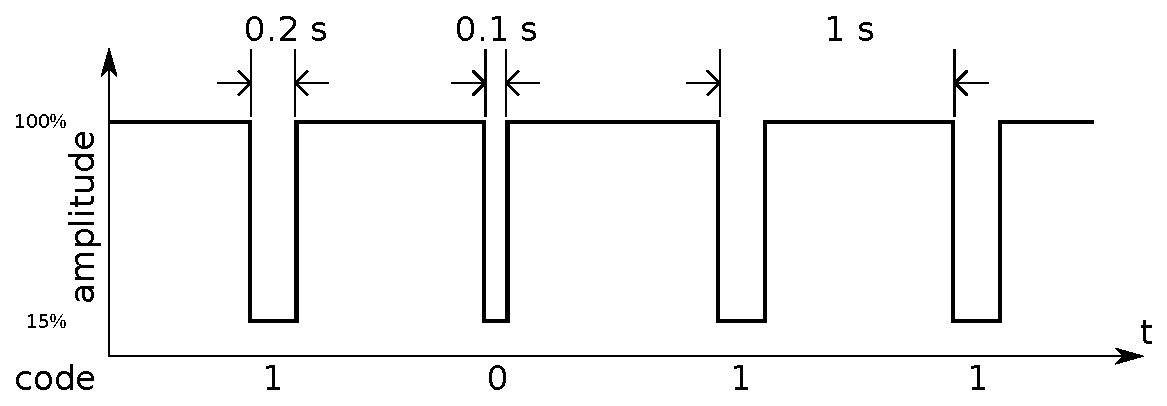
\includegraphics[width=0.8\linewidth]{DCF77_code.pdf}
\caption{Modulace signálu z~vysílače DCF77.}
\end{figure}

V~59 bitech jsou kódovány např.
\begin{itemize}
	\setlength{\itemsep}{1pt}
	\setlength{\parskip}{0pt}
	\setlength{\parsep}{0pt}

	\item datum,
	\item čas,
	\item zda běží letní nebo zimní čas, nebo
	\item všemožná varování před katastrofami, počasí.
\end{itemize}

Význam jednotlivých bitů zde nebudu popisovat, je snadno dohledatelný buď na
internetu, nebo pochopitelný přímo z~implementace (viz \texttt{dcf.h}).

%%%%%%%%%%%%%%%%%%%%%%%%%%%%%%%%%%%%%%%%%%%%%%%%%%%%%%%%%%%
\section{Zapojení hardware}

Přijímač signálu DCF77 je připojen k~napájení +5V, datový vodič je připojen na
pin PD3.

Obvod RTC je připojen na piny PD0 (SCL), PD1 (SDA) a PD2 (INT).

Žádný další hardware není nutný.

%%%%%%%%%%%%%%%%%%%%%%%%%%%%%%%%%%%%%%%%%%%%%%%%%%%%%%%%%%%
\section{Popis činnosti}

Přiložená implementace po startu vyčkává na začátek celé minuty, pak zahájí
příjem oněch 59 bitů. Po přijetí zprávy zajistí uložení aktuálního data
a času do modulu RTC. Firmware průběžně posílá informace o~stavu příjmu dat na
sériovou linku s~rychlostí 9600 baud.

%%%%%%%%%%%%%%%%%%%%%%%%%%%%%%%%%%%%%%%%%%%%%%%%%%%%%%%%%%%
\section{Implementace}

Firmware je psaný modulárně, každý soubor se stará vždy o~jednu věc:
\begin{itemize}
	\setlength{\itemsep}{1pt}
	\setlength{\parskip}{0pt}
	\setlength{\parsep}{0pt}

	\item \texttt{dfc.h}, \texttt{dcf.c}: příjem signálu z~DCF,
	\item \texttt{rtc.h}, \texttt{rtc.c}: komunikace s~modulem RTC,
	\item \texttt{i2c.h}, \texttt{i2c.c}: funkce pro komunikaci přes I2C
		(využito pro RTC),
	\item \texttt{serial.h}, \texttt{serial.c}: komunikace přes sériovou linku,
	\item \texttt{bcd.h}: pomocné funkce pro převod mezi BCD a běžným kódováním,
	\item \texttt{main.c}: spojení všech modulů.
\end{itemize}

Vyhodnocování signálu z~modulu DCF77 je psáno s~důrazem na odolnost proti rušení
a na rychlost. V~praxi to znamená například to, že hrana indikující začátek sekundy
je napojena přímo na přerušení. V~tomto přerušení dojde k zaznamenání času,
program pak počká cca 120 ms a v~dalších 80 ms každou milisekndu měří, jaká
je logická hodnota na vstupu signálu z~vysílače. Pokud v~oněch 80 naměřených
hodnotách výrazně převáží signál HIGH, nebo LOW, je tento bit započten. Pokud
vlivem rušení signál \uv{přeskakuje} mezi jednotlivými hodnotami nad únosnou
míru, je bit vyhodnocen jako neplatný a celá zpráva ignorována. V~praxi se
ukázalo, že tento způsob příjmu signálu je poměrně odolný vůči občasným
fluktuacím na vstupu.

%%%%%%%%%%%%%%%%%%%%%%%%%%%%%%%%%%%%%%%%%%%%%%%%%%%%%%%%%%%
\section{Diskuze}

Původní myšlenka příjmu signálu zahrnovala ještě mechanismus, který neměl
v~případě nemožnosti dekódovat bit (vlivem rušení) zapomínat celou zprávu,
ale jen si poznačit, že tento konkrétní bit nebyl správně dekódován a vzít
jej z~příští zprávy. Tento nápad zásadně (!) snižuje čas potřebný
k~dekódování celé zprávy, problém je ale v~tom, že bity se mezi jednotlivými
minutami mění. Nelze tedy (jednoduše) říci \uv{5 z~58 bitů se mi nepodařilo
dekódovat, tak si je doplním v~další minutě a mám hotovo}.

Pokud by se chtělo vytvořit skutečně robustní systém, mělo by se ale toto
\textit{postupné skládání bitů} uvážit a implementovat, avšak je potřeba
promyslet, jak to udělat, aby byla přijatá informace konzistentní.

\end{document}
